\listfiles
\documentclass[a4paper, oneside]{report}

\usepackage[utf8]{inputenc}
\usepackage[francais]{babel}

\usepackage{amssymb}

\usepackage[pdftex]{graphicx}
\usepackage{graphics}

\usepackage[top=3cm, bottom=2cm, left=3cm, right=2cm]{geometry}

\usepackage{multirow}
\usepackage{tabularx}

\usepackage{listings} % a inclure pour la fonction listing
\usepackage{color} % on en a besoin pour utiliser les couleurs
\definecolor{grey}{rgb}{0.95,0.95,0.95} % on definit la couleur grise (c'est un gris tres clair)
		
\usepackage{float}

\renewcommand{\floatpagefraction}{.9} 
%utilisee avec la commande :
\renewcommand{\textfraction}{.1}
%permet de dire que le texte peut n'occuper que 10% d'une
%page, et donc que des flottants peuvent occuper les 90% restant.


%Il y a d'autres parametres interessants :
\setcounter{totalnumber}{4} 
\setcounter{secnumdepth}{3}
%qui determine le nombre de flottants autorises par page,
\renewcommand{\topfraction}{.8}
\renewcommand{\bottomfraction}{.8}

\lstset{numbers=left, tabsize=2, frame=single, breaklines=true, basicstyle=\ttfamily, numberstyle=\tiny\ttfamily, framexleftmargin=13mm, backgroundcolor=\color{grey}, xleftmargin=12mm}

% titre du document
\title{IN41 \\TP5 : Filtrage d'un signal num\'erique}
% auteur du document
\author{Ripard Maxime}

\begin{document}
  \maketitle
  \newpage{}
  \tableofcontents
  \newpage{}

  \chapter{Lecteur et enregistrement des fichiers audios}
  
On r\'ecup\`ere la valeur de chaque signal temporel ainsi que sa fr\'equence d'\'echantillonage via la fonction $waveread$ de Matlab.\\
La fonction $wavplay$ nous permet de lire ces fichiers son.\\

\begin{lstlisting}
function [ ] = Untitled( filename )

%Ouverture du fichier son
[yt, F,N] = wavread(filename);

%Ecoute du fichier
wavplay(yt,F);
  \end{lstlisting}
    
 \chapter{Analyse spectrale du signal audio num\'erique avec ou sans bruitage}

\section{Bornes et fr\'equence du signal}

Nous calculons les bornes et fr\'equences des signaux gr\^ace au code suivant.

\begin{lstlisting}
% bornes et frequence du signal
f=linspace(-fe/2,fe/2,length(y));

size = wavread(filename,'size');
t = [0:size-1];
\end{lstlisting}

\vsize 0,5 cm

\section{Calcul de la TFD}

On calcule la transform\'ee de fourier discr\`ete avec le code suivant : \\

\begin{lstlisting}
% Calcul de la TFD du signal
yf = fftshift(fft(yt));
\end{lstlisting}

\vsize 0,5 cm

\section{Application de bruit}

On applique notre bruit sur le signal : \\

\begin{lstlisting}
%Cr\'eation du bruit avec y le signal cr\'e\'e pr\'ec\'edemment
bruit=(var(yt)).*randn(length(yt),1);
%Ajout du bruit au signal sonore
ytB=yt+bruit;
\end{lstlisting}

On enregistre les nouveaux signaux sur lesquels on a rajout\'e le bruit : \\

\begin{lstlisting}
% on enregistre le signal avec le bruit
wavwrite(ytB,F,N,strcat('bruit_',filename));        
\end{lstlisting}

\newpage{}

\section{Calcul de la TFD du signal bruit\'e}

\begin{lstlisting}
% Calcul de la TFD du signal sonore avec le bruit
yfB=fftshift(fft(ytB));
\end{lstlisting}

\begin{lstlisting}
% Representation du signal initial et avec le bruit
figure(1);

subplot(4,1,1);
plot(t,ytB,'r',t,yt,'b');
title('Signal temporel');
legend('signal+bruit','signal');
xlabel('t');
ylabel('Amplitude');
\end{lstlisting}

  \begin{figure}[h]
 \centering
 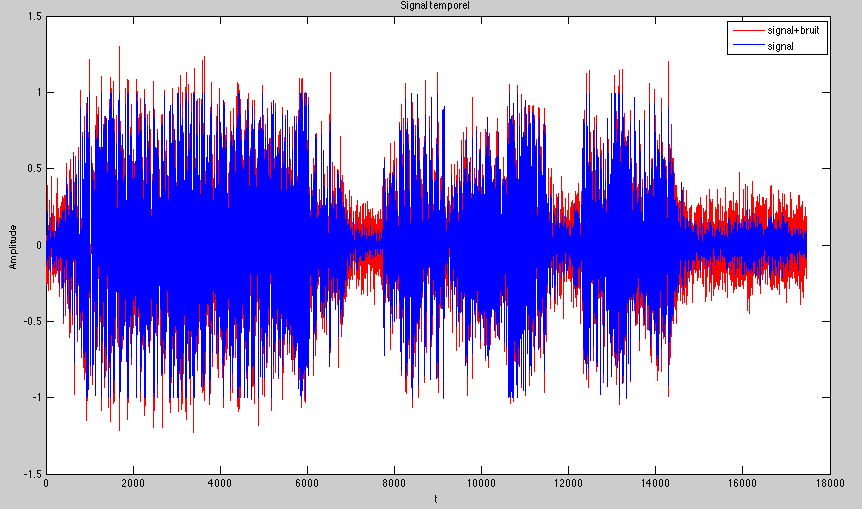
\includegraphics[scale=0.42]{images/source_bruit.png}
 \caption{Repr\'esentation du signal sonore avec et sans le bruit}
 \end{figure}
 
 \begin{figure}[h]
 \centering
 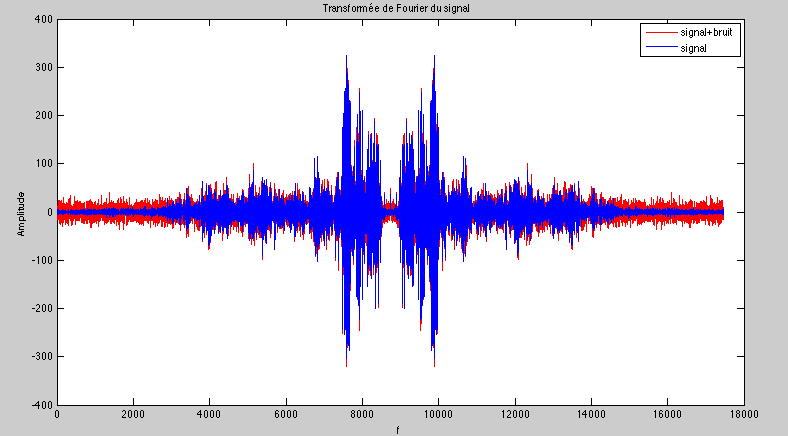
\includegraphics[scale=0.5]{images/signal_bruit_fft.png}
 \caption{Repr\'esentation du signal sonore ayant subi une fft, avec et sans le bruit}
 \end{figure}
  
  \newpage{}
  
 \section{Analyse des fr\'equences \`a filtrer}
 
 Sur le signal 1, le bruit affecte \'enorm\'ement le signal, \'etant pr\'esent dans toutes les fr\'equences, et toutes les gammes de fr\'equences.\\
 
 Le signal 2 lui est affect\'e par le bruit principalement dans les fr\'equences hautes au dessus de 2 kHz. Le bruit affecte peu le reste des fr\'equences et notamment les lobes principaux, qui nous sont particuli\`erement utiles car ils contiennent la plupart des informations utiles du signal.

 \section{Application des filtres}
 
Nous utiliserons les filtres des TP3 et 4, et essentiellement celui de Butterworth, car nous avions conclu que celui ci \'etait meilleur que celui de Chebyshef. Par des tests, nous nous sommes rendus compte qu'un filtre d'ordre 24 \'etait suffisamment pr\'ecis sans pour autant n\'ecessiter de lourds calculs.

\begin{lstlisting}
%On cree les constantes necessaires pour le filtrage
Fc=size(1)/2;
BP=3000;

w=2*pi*t;
Wn=[2*pi*(Fc-(BP/2)) 2*pi*(Fc+(BP/2))];

%Creation et application du filtre
[D,C]=butter_asi(12,Wn,'bandpass','s');
HfButter=freqs_asi(D,C,w);
HfButter=abs(HfButter);
yfF=yfB.*HfButter';
\end{lstlisting}

\begin{lstlisting}
plot(t,real(yfF));
title('Signal filtr\'e');
xlabel('f');
ylabel('Amplitude');
\end{lstlisting}
 
 \newpage{}
 
 \section{Interpr\'etation des r\'esultats}
 
 \begin{figure}[h]
 \centering
 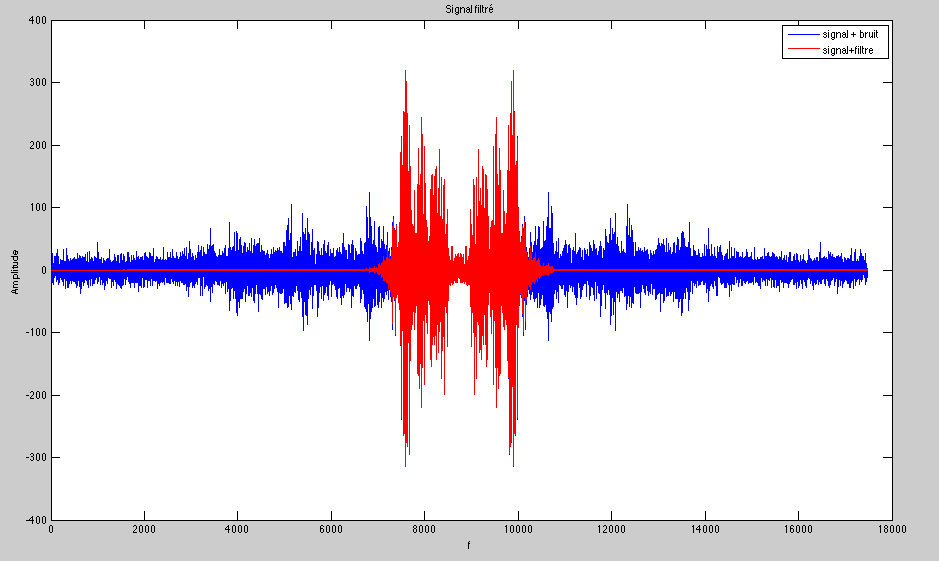
\includegraphics[scale=0.42]{images/filtre.png}
 \caption{Analyse spectrale du signal  debruit\'e en superposition avec le signal original}
 \end{figure}
  
 On s'aper\c coit ici que une grande partie du signal a \'et\'e tronqu\'ee, sans pour autant d\'et\'erirorer les lobes, source majoritaire de l'information dans le signal.\\
 
 
 Faire varier les param\`etres change le filtrage, n\'eanmoins, l'ordre le plus grand possible est toujours un bon choix. Le choix est ici plus discutable sur la bande passante, mais comme je l'ai expliqu\'e plus haut, il est n\'ecessaire de la choisir relativement grande, mais pas trop, afin d'\'eliminer le bruit en conservant le signal.

 \chapter{Bilan}
 
\begin{lstlisting}
ytF = ifft(yfF);
wavwrite(ytF,F,N,'filtre.wav');

% subplot (4,1,4);
plot(t,real(ytB),'r',t,real(ytF),'b');
title('Signal bruit\'e et signal reconstitu\'e');
legend('signal+bruit','signal');
xlabel('t');
ylabel('Amplitude');
\end{lstlisting}

 \begin{figure}[h]
 \centering
 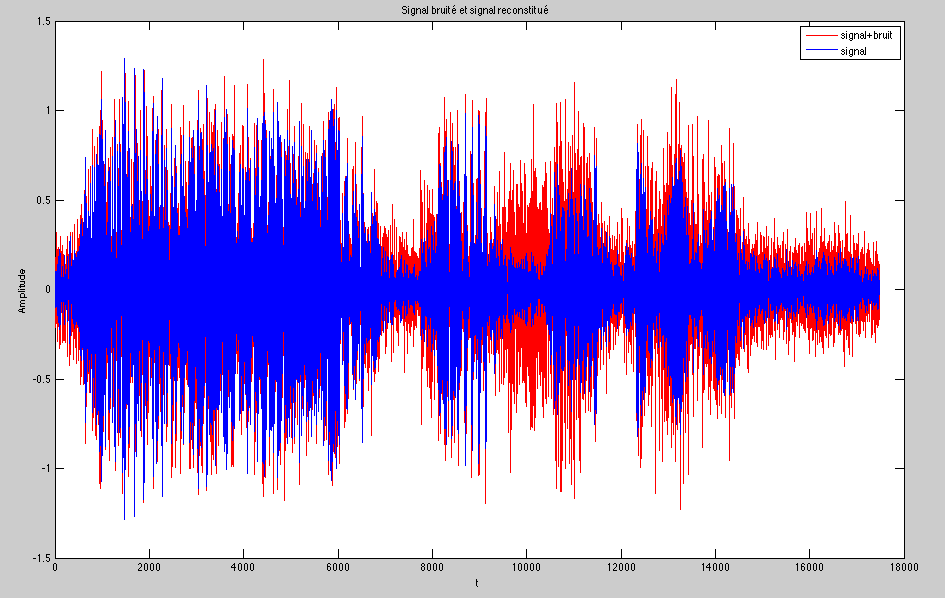
\includegraphics[scale=0.42]{images/signal_reconstitue.png}
 \caption{Analyse spectrale du signal  debruit\'e en superposition avec le signal original}
 \end{figure}

On voit ici que le signal a \'et\'e tr\`es fortement nettoy\'e du bruit qui y \'etait pr\'esent. Le bruit n'a pas compl\`etement disparu, mais la majorit\'e des lobes a \'et\'e pr\'eserv\'e. Le filtrage n'est donc certes pas parfait, mais il est efficace.

\end{document}